
\lab{Applications}{Monte-Carlo Integration}{Monte-Carlo Integration}

\objective{This section explains the basics of Monte-Carlo Integration.}

Integration is important in a variety of applications. However, high-dimensional integration is highly inefficient using the standard one-dimensional methods. Accordingly, we are forced to pursue a different method. The method of choice in high dimensional settings is known as Monte-Carlo Integration, and is based upon random sampling. This technique is applied in a large variety of fields, such as optimization, physics, and finance.

Consider the following example: Suppose our goal is to estimate the area of a circle (we select this problem because it has a closed form solution, which we can use to test the method). One method that we could use for empirically finding that area is to throw darts randomly at a square board. We then can find the area of the circle by multiplying the square's area by the percentage of darts that fell in the inscribed circle. We can do this using the following code (the resulting figure is shown in Figure \ref{Fig:MCCircle}).


\begin{lstlisting}[style=python]
numPoints = 500
points = sp.rand(numPoints,2)
points = 2*(points-.5)
pointsNorm = sp.hypot(points[:,0],points[:,1])
InCircle = sp.nonzero(pointsNorm < 1)
OutCircle = sp.nonzero(pointsNorm > 1)
plt.plot(points[InCircle,0],points[InCircle,1],'r.');
plt.plot(points[OutCircle,0],points[OutCircle,1],'b.');

#Plots a Circle
theta = sp.linspace(0,2*sp.pi,50)
plt.plot(sp.cos(theta),sp.sin(theta),'k')

plt.axis('off');
plt.axis('equal');

plt.show()

area = 4.0*sp.size(InCircle)/numPoints

\end{lstlisting}

\begin{figure}[h!]
\begin{center}
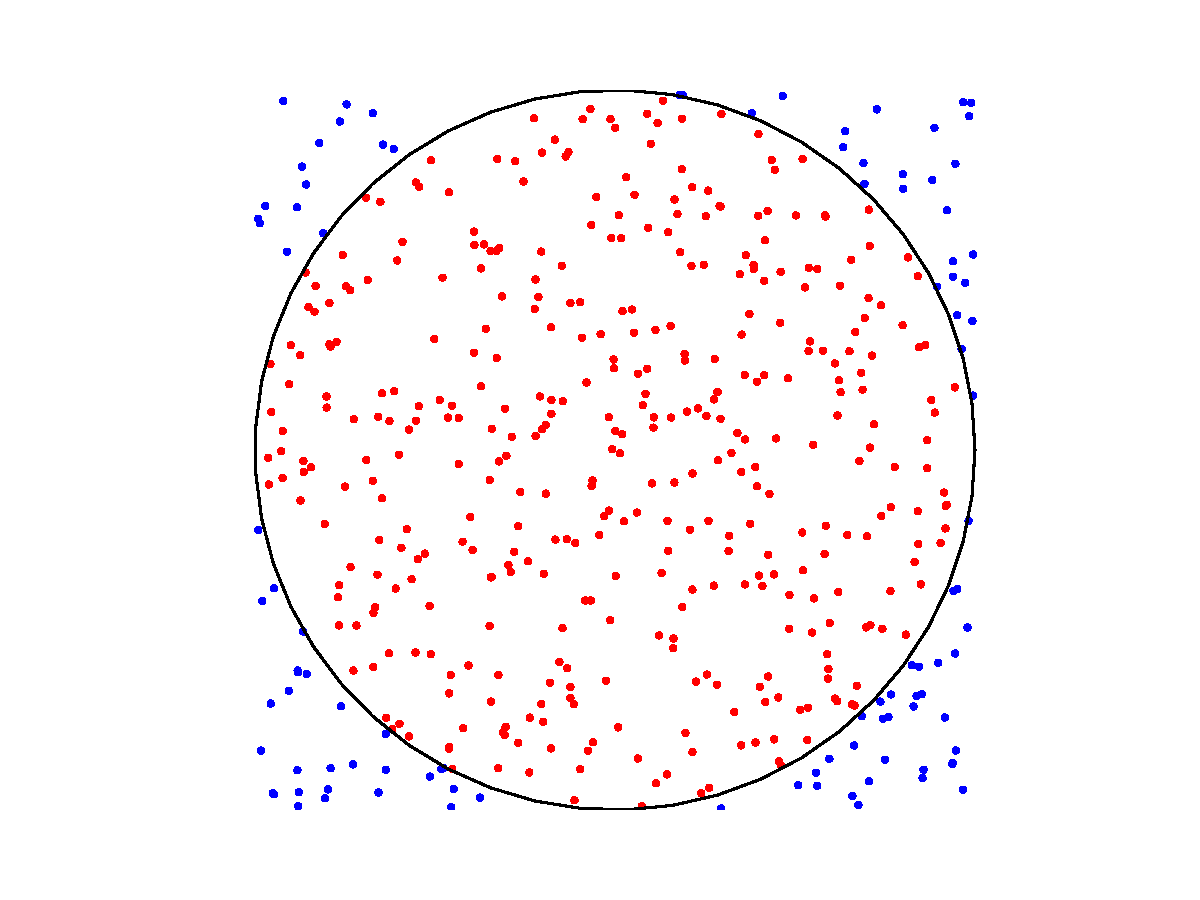
\includegraphics[scale = .4]{MCCircle}
\caption{Finding the area of a circle using random points}
\label{Fig:MCCircle}
\end{center}
\end{figure}

In this case the area should be $\pi$, and the approximation is pretty good.

One important question is the rate at which our estimate converges. We can test this using a log plot using the following code:
\begin{lstlisting}[style=python]
numTestPoints = 29;
testPoints=sp.around(sp.linspace(1000,100000,numTestPoints))
error = sp.zeros(sp.size(testPoints))
testRuns=100
area = sp.zeros(testRuns)

for i in range(0,numTestPoints):
	for k in range(0,testRuns):
		numPoints = testPoints[i]
		points = sp.rand(numPoints,2)
		points = 2*(points-.5)
		pointsNorm = sp.hypot(points[:,0],points[:,1])
		inCircle = sp.count_nonzero(pointsNorm < 1)
		area[k] = 4.0*inCircle/numPoints
	error[i] = sp.mean(sp.absolute(area-sp.pi))
sp.size(error)
sp.size(testPoints)

plt.plot(sp.log(testPoints),sp.log(error));
estimate = la.lstsq(sp.vstack((sp.log(testPoints),sp.ones(sp.size(testPoints)))).T,sp.log(error))
convergenceRate = estimate[0][0]
\end{lstlisting}

Note that we estimate the convergence rate using Least Squares, as in Lab \ref{Stats1}. The rate should be something like $-.5$. This means that the estimate of the error improves as $1/\sqrt{N}$, meaning that to improve our error estimate by 10 times (one digit) we must sample 100 times more points. This is not a very desirable convergence rate. However, this rate is independent of the number of dimensions (a property not shared by one-dimensional integration techniques), and is therefore desirable for high-dimensional problems.

The problem of calculating the area of a circle above can actually be reformulated as the following integration problem:
\[
\mbox{Estimate }A = \int_{[-1,1]\times[-1,1]} f(x,y)
\]
where
\[
f(x,y) = \begin{cases} 1 &\mbox{ if $x$ is in the unit circle} \\ 0 &\mbox{ otherwise} \end{cases}
\]

Using a similar method we can actually solve any integration problem. Suppose that we desire to solve the integral
\[
\int_\Omega f(x)
\]

Where $x$ is a vector and $\Omega$ is a region. We can approximate the integral using the formula
\[
\int_\Omega f(x) \approx V(\Omega) \frac{1}{N} \sum_{i=1}^N f(x_i)
\]

Where $x_i$ are uniformily distributed random vectors in $\Omega$, and $V$ gives the volume of a region. This formula exactly describes how to perform Monte Carlo Integration.

\begin{problem}
\label{prob:mc}
Write code implementing Monte Carlo Integration on the unit square for an arbitrary input function. You may require that the user input the number of dimensions. Allow the user to input the number of points to use as well.
\end{problem}

\begin{problem}
\label{prob:mc_test}
Test your solution to Problem \ref{prob:mc}, and the convergence of the method, on the function:
\[
f(w,x,y,z) = sin(x) y^5 -y^3 + zw + yz^3
\]
This integral should converge to zero. Estimate the exponent of convergence (it should be close to $-.5$)
\end{problem}

We note that we must use caution in using monte carlo integration when we don't know if the integral actually converges to a finite value. For example the following integral does not converge(is not finite):
\[
\int_0^1 \frac{1}{x}
\]

We can attempt Monte Carlo Integration on such an integrand using the following code:
\begin{lstlisting}[style=python]
k = 5000
sp.mean(1/sp.rand(k,1))
\end{lstlisting}

We will get a finite value in return, so we could assume (incorrectly) that this integral has a finite value. However, by experimenting with larger values of $k$ you will notice that the integral does not converge to a specific value, which is because the actual integral does not converge. Therefore it is often important to understand some of the properties of the integrand analytically prior to using this type of integration.

Another important key to successful Monte Carlo integration are that the random numbers be uniformily distributed. If they are not, our answer will not converge to a correct answer. This is one of the reason that good pseudo-random number generators are so important.

\begin{problem}
\label{prob:mc_flawed}
Create a new function (based upon the function from Problem \ref{prob:mc}) that uses a ``flawed'' random number generator that doesn't produce numbers between $-.95$ and $-1$. Test your method on the function from Problem \ref{prob:mc_test}. How bad is the error? 
\end{problem}




%
%{\bf Outline:}
%
%\begin{itemize}
%\item Background: High Dimensional Integration is hard. Standard methods can have a hard time focusing on important areas. As we add dimensions we have to sample a lot more points (it adds an order of difficulty)
%\item Toy Example: Area of a shape? Throwing Darts...
%\item Demonstrate how the error decreases ($1/\sqrt{N}$).
%\item Talk about adaptive methods? Give example of how to do this in 1D. This will touch on Approximation Theory. Probably better in the Variance Reduction section.
%\end{itemize}
%
%\begin{problem}
%Calculate a simple 1D problem (maybe using the code for simple newton-cotes from earlier?). Compare convergence with {\tt quad}. Quantify advantages(keep using old data easily). Plot error.
%\end{problem}
%
%\begin{problem}
%Use MC integration to calculate a higher dimensional integral. Maybe a random many-D high order polynomial, or a function we know should go to zero (high order odd function?)
%\end{problem}
%
%{\bf Other possible options (more material/problems)}
%
%\begin{problem}
%Explain Asian Options briefly. Show how to calculate their value using MC techniques.
%\end{problem}
%
%\begin{problem}
%Buffoon's Needle (A simple empirical way to calculate $\pi$) can be formulated as a Monte-Carlo Integration problem. This could be a simulated/experiment lab.
%\end{problem}
%
%\begin{problem}
%Demonstrate need for good ``random'' variables for MC integration to work (maybe use a delibarately flawed prng on the high-dimensional problem above). One more recent test developed for random variables is based on picking subspaces and testing randomness (I think this is in Knuth), we can talk about how this type of flaw applies to MC integration.
%\end{problem}
